\section{Construction}\label{sec:construction}

\subsection{The Setting}

We are given $n \in \mathbb{N}$ ledger protocols
$\Y[][1], \Y[][2], \ldots, \Y[][i], \ldots, \Y[][n]$,
the so-called \emph{underlying} ledger protocols.
While mathematically, these $\Y$s are interactive Turing machines of ledger protocols,
in practice, these are preexisting, already operational ledger protocol executions
such as Bitcoin, Ethereum, and Cardano, for which we have access to already running full nodes
and we are asked to compose on top of.

We are also given a distributed protocol $\Pi$ (not necessarily a ledger protocol),
the so-called \emph{overlay} protocol. We will simulate an $n$-party execution of $\Pi$,
with each $i$ of these $n$ parties corresponding to the underlying ledger protocol $\Y[][i]$.

The users of the protocol are $m \in \mathbb{N}$ \rollerblade \emph{clients} termed
$\RB[1], \RB[2], \ldots, \RB[j], \ldots, \RB[m]$ (with, potentially $m \neq n$).
\emph{Each} $\RB[j]$ client runs a separate full node $\Y[j][1], \ldots, \Y[j][i], \ldots, \Y[j][n]$
for each of the underlying $\Y$s. The $\RB$ nodes do not have direct network communication, but only
use the read/write functionalities of their respective $\Y$ instances to communicate.
For example, when party $\RB[1]$ \emph{writes} a transaction $\tx$ to its $\Y[1][1]$ instance,
this transaction will eventually appear in $\RB[2]$'s $\Y[2][1]$ instance ledger output,
as long as $\Y[][1]$ is live.
We will use $\Ledger[j][i][r] \gets \Y[j][i][r].\lread()$ to refer to the ledger reported at
round $r$ by the full node instance $\Y[j][i]$ running the underlying ledger protocol $\Y[][i]$
operated by the overlay party $\RB[j]$
(this ledger, like all ledgers, is a sequence of round/transaction pairs, and its
$k^\text{th}$ round/transaction pair is $\Ledger[j][i][r][k]$).
%
% TODO: move this to consensus section
% Our goal is to build a \emph{new} DLP $\RB$
% on top of these such that, if the majority of \emph{underlying}
% $\wheel[1], \ldots, \wheel[n]$ are \emph{secure}, then so is the
% \emph{overlay} DLP $\RB$. As $\RB$ is a DLP, it will have its own population of $m$ nodes
% $\RB_1, \RB_2, \ldots, \RB_m$. The $\RB$ DLP will have its own type of transaction and a
% ledger consisting of these transactions. For example, it can maintain its own coin\footnote{
% We will not be concerned with bridging this coin from the overlay ledger to the underlying
% ledgers. This can be done using various standard bridging techniques which are orthogonal
% to this work~\cite{pow-sidechains,pos-sidechains,zkbridge}.}. Importantly, similarly to
% a rollup, \emph{we will not make any additional security assumptions about the honesty of the
% $\RB$ nodes}.

% \textbf{Bulletins.}
% We do not want to modify the underlying DLPs to support our protocol. However, the underlying DLPs
% do not understand the transaction semantics of our overlay ledger. We will therefore use the underlying
% DLPs as a simple lazy transaction ordering service. We will assume that we can take any
% arbitrary string $w$ and \emph{encode} it into a transaction suitable for each underlying ledger.
% Such transactions are \emph{always} accepted by the underlying ledger, and their contents
% are not validated (beyond checking that a minimum fee is suitably paid to avoid spamming attacks).
% We call a DLP that supports writing such arbitrary data into it a \emph{bulletin}. A bulletin
% DLP offers two additional functions $\tx \gets \textsf{encode}(s)$ and $s \gets \textsf{decode}(\tx)$.
% The $\textsf{encode}$ function one takes a string $s$ and encodes it into a transaction $\tx$ that can be \emph{written}
% into the DLP and is guaranteed to be accepted. The $\textsf{decode}$ function takes a transaction $\tx$
% and, if it is a bulletin transaction, decodes it back into $s$. Otherwise, $\textsf{decode}$ can return $\bot$.
% All transactions produced by $\textsf{encode}$
% are bulletin transactions, but the adversary can also introduce arbitrary bulletin transactions of her choice
% indiscriminately. The DLP may also include non-bulletin transactions among the bulletin transactions.
%
% \begin{definition}[Bulletin]
%   A DLP $\Pi$ accompanied by a pair of functions $(\textsf{encode}, \textsf{decode})$,
%   is called a \emph{bulletin}. It must hold that, for any $s \in \{0, 1\}^*$,
%   the output of $\tx = \textsf{encode}(s)$ is always a valid
%   transaction and that $\textsf{decode}(\textsf{encode}(s)) = s$.
% \end{definition}
%
% % TODO: Require that "encode" produces a high-entropy transaction
% % so that we know that honest relayers will produce new honest transactions
% % in every round, and the Past Perfect conjecture will follow.
%
% Bulletins provide ordering and data availability of arbitrary data without checking
% any semantic validity. As such, they constitute a \emph{lazy} use of a ledger~\cite{lazyledger,lazylight}.
% All popular blockchains such as, for example, Ethereum and Bitcoin are bulletins.
% Bitcoin allows the recording of arbitrary data using \textsf{OP\_RETURN}
% transactions, whereas Ethereum allows such recording by including the
% data in the \textsf{CALLDATA} of a smart contract call, or in the parameters
% of an event.
%
% \subsection{A Majority Vote}\label{sec:construction-naive}
%
% Composing many underlying ledgers into an overlay ledger is not complicated, but it is complex
% protocol, with many moving parts. As such, we present the design in iterative stages. In the
% first stage, presented in the present section, we provide a design based on an \emph{honest majority}
% approach. This obvious approach introduces the notation and allows us to familiarize the reader
% with the concepts, but is ultimately misguided. However, it is imperative for understanding why
% a straightforward solution is not applicable, and a stepping stone for the next development in
% the protocol. In the section that follows, we introduce a BFT layer running on top of our
% underlying ledgers. This is our final construction, but we describe it intuitively first before
% we delve into the technical details of a precisely defined construction in the next section.
% We leave the formal analysis and proofs of security for the end.
%
% The first and obvious approach to compose ledgers starts by the assumption that the
% underlying majority is secure. The core idea is to produce the overlay ledger by taking
% a majority vote on the reported underlying ledgers. The construction is illustrated in
% Figure~\ref{fig.naive}, where
% $m$ parties $\RB[1], \ldots, \RB[m]$ run the overlay protocol.
% Each of the $\RB$ nodes runs
% a full node to each of the $n$ underlying DLPs $\wheel[1], \ldots, \wheel[n]$, pictured as squares
% of varying shades of yellow. The full nodes communicate with one another using their
% respective DLP technology, which we treat as a black box here, depicted as elongated
% rectangles in varying shades of red towards the bottom of the figure.
% The $\RB$ nodes
% make their own overlay DLP, offering \emph{read} and \emph{write} functionalities.
%
% \begin{figure*}
%     \centering
%     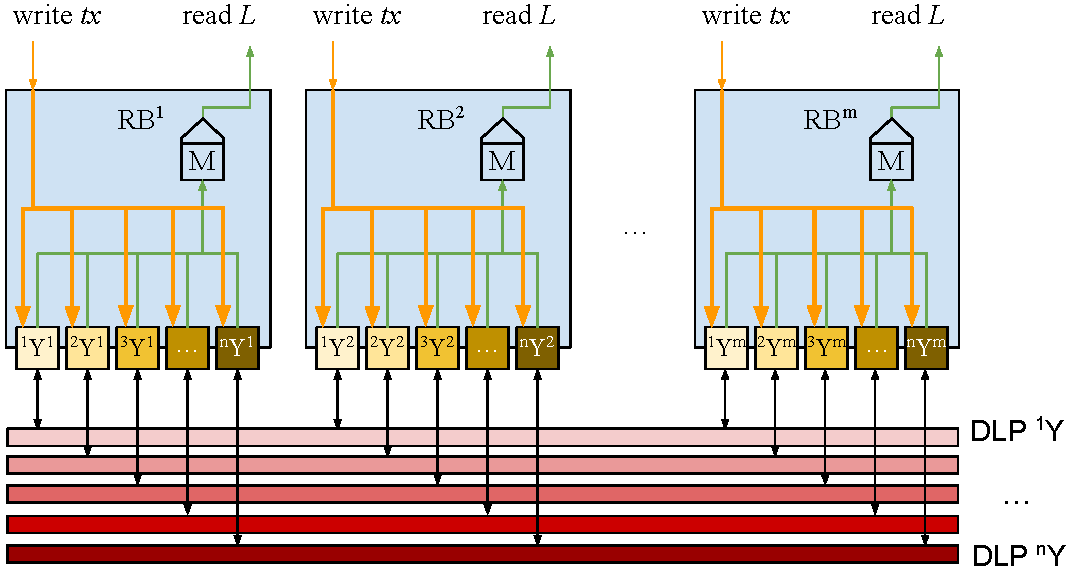
\includegraphics[width=\textwidth,keepaspectratio]{figures/rollerblade-naive-construction.pdf}
%     \caption{The first attempt at the composed construction. Here,
%              $m$ different parties $\RB_1, \ldots, \RB_m$ operate Rollerblade
%              nodes, each of which runs a client on $n$ different underlying
%              DLPs $Y_1, \ldots, Y_n$.}
%     \label{fig.naive}
% \end{figure*}
%
% When an $\RB$ transaction $\tx$ is \emph{written} into one of the $\RB$ nodes by the user,
% the $\RB$ serializes this transaction for each of the underlying DLPs (using the
% serialization mechanism particular to each individual DLP) and posts it
% as a transaction there, depicted as orange wires running downwards in the figure.
% Let us walk through
% this process precisely.
% The $\RB$ party takes $\tx$ and wraps it in a \emph{message}
% which is the pair $m = (`\text{write}', \tx)$.
% This captures the user intent to \emph{write} this overlay transaction to the underlying ledgers.
% The first element of the pair (\emph{`write'}) indicates the \emph{type} of message.
% As we evolve our protocol, we will introduce other control message types later, but,
% for now, this is our only message type. Once the message is created, we pass it to
% \textsf{encodeRollerbladeTx}, listed in Algorithm~\ref{alg.encode}.
% This function first serializes $m$
% into a string $s = \textsf{serialize}(m)$. This string is then encoded for each particular
% underlying DLP $\wheel[i]$ by invoking the bulletin functionality $\wheel[i]\text{.encode}$.
% This returns a transaction $\tx'_j$, which is appropriate for being written to $\wheel[i]$.
% Note that $\tx$ is a transaction of the overlay ledger, whereas each of $\tx'_i$ is a
% transaction of the underlying ledger $\wheel[i]$. Each resulting underlying transaction $\tx'_i$
% is then broadcast into $\wheel[i][j]$ by having $\RB[j]$ invoke the \emph{write}
% functionality of $\wheel[i][j]$.
%
% \import{./}{algorithms/alg-encode}
%
% Each transaction $\tx'_i$ is written to the respective underlying DLP $\wheel[i][j]$ during
% the same round $r$. If $i$ happens to be live, the respective \emph{read} call of all
% other $j'$ DLPs on $\wheel[i][j']$ at round $r' \geq r + u$ will result in a ledger
% $\wheel[i][j'][r']$ containing $\tx'_i$.
%
% In order to answer a particular overlay \emph{read} call, the overlay party $\RB[j']$ must
% issue a \emph{read} to all of its underlying DLPs $\wheel[1][j'], \ldots, \wheel[n][j']$,
% depicted as green wires running upwards in the figure.
% The transactions in $\wheel[i][j'][r']$ are of $\wheel[i]$ format,
% and therefore must be decoded using the bulletin decoding functionality
% appropriate to each underlying DLP $\wheel[i]$.
% Those that decode successfully result in a string $s$ which can, in turn,
% be deserialized into a message $m = (`write', \tx)$ containing the type \emph{`write'}
% and the overlay transaction $\tx$. The process of decoding and deserializing a transaction
% is done through the \textsf{decodeRollerbladeTx} algorithm, listed in Algorithm~\ref{alg.encode}.
% It invokes \textsf{decodeRollerbladeTx} in each of the returned ledgers, resulting
% in a sequence of $n$ ledgers $\overline{L}$, each a sequence of overlay transactions.
% We call this process \emph{sanitization} and list it in Algorithm~\ref{alg.sanitize}.
%
%
% Next, the overlay party $\RB[j']$ will need a mechanism to combine these sanitized ledgers
% into \emph{one} ledger in order to answer the \emph{read} call from the user.
% The sanitized ledgers are fed into a \emph{majority voting} contraption, denoted with
% the letter M and the \emph{house} symbol in the figure, which then outputs the desired
% ledger $L$ of $\RB$ transactions (top).
% The idea is that, if the majority of underlying ledgers is secure, the transaction $\tx$
% in question will eventually appear (liveness) and stabilize (safety) in a majority of them.
% The party $\RB[j']$ can therefore take a majority vote among the underlying ledgers
% to extract an overlay ledger aspiring to be safe and live.
% The algorithm listed in Algorithm~\ref{alg.majorityvote} performs the majority voting
% process. It is invoked when the user of $\RB[j]$ invokes \emph{read} at a certain
% round $r$. The process accepts a list of ledgers $\overline{L}$ each $\prescript{i}{}{\overline{L}}$
% of which contains the sanitization of the underlying ledger $\wheel[i][j][r]$.
% The majority of $\overline{L}$ will contain all the honest
% transactions issued at least $u$ rounds ago. It goes through each
% position in the sanitized ledgers. For each position $k \in \mathbb{N}$,
% it observes what each of the $n$ ledgers report in the $k^\text{th}$ position.
% The reported transactions in the $k^\text{th}$ position are
% $\wheel[1][j][r][k], \wheel[2][j][r][k], \ldots, \wheel[n][j][r][k]$.
% The algorithm counts the frequency of appearance of each transaction at
% the position $k$. If a transaction
% appears more than $\frac{n}{2}$ times in this position, it is included in the sanitized ledger
% (since we have $n$ underlying ledgers, only one transaction can do so).
% Otherwise, if no transaction appears more than $\frac{n}{2}$, the sanitized ledger
% is cut short and returned.
%
% \import{./}{algorithms/alg-majorityvote}
%
% The intuition why this majority voting \emph{should work} is this: An honest
% transaction will eventually be included in all of the underlying ledgers that
% are live, and hence will appear in more than $\frac{n}{2}$ underlying ledgers
% and will make it to the output of \textsf{MajorityVote}. Since the majority
% of underlying ledgers is secure, they will maintain the transaction order,
% and so will the output of \textsf{MajorityVote}. In order for the adversary
% to censor a transaction from the final ledger, the adversary will need to
% break the security of more than $\frac{n}{2}$ underlying ledgers.
%
% Unfortunately, this argument does not hold water. The reason is that, due to
% delays, two transactions $\tx_1$ and $\tx_2$ may appear in a different order
% in different underlying ledgers, even if all of them are secure. It is possible
% that $\tx_1$ appears before $\tx_2$ in $\lfloor \frac{n}{2} \rfloor$ of the
% underlying ledgers, whereas it appears after $\tx_2$ in the $\lceil \frac{n}{2} \rceil$
% of the rest\footnote{In fact, it is possible, even with every underlying ledger being
% secure, that each ledger reports a particular order of transactions, but the majority voting
% cannot not result in an order at all. This is known as a Condorcet cycle~\cite{condorcet}.}.
% The adversary can then easily swap the transaction order by
% breaking the security of only one chain. Therefore, this initial design
% is not secure. We are now ready to rectify this issue by introducing a more
% nuanced mechanism in place of majority voting.
%
% \subsection{A BFT to Rule Them All}\label{sec:construction-bft}
%
% \begin{itemize}
%   \item Simple majority voting construction with no BFT protocol on top. Serialization and deserialization requirements and algorithms. Majority voting on ``ledger extensions'' algorithm. Fragile results in which different blockchains can disagree on the order and one blockchain can ``flip over'' the result. l. Condorcet cycles.
%   \item The necessity of running a BFT protocol on top, but without talking about the oracle abstraction of signatures, broadcasting, verification, and receiving. Light clients from one blockchain to another using smart contracts. Using the blockchains as ports of communication.
%   \item Oraclizing sign/broadcast and receive/verify.
%   \item Remove the smart contract assumption using dirty ledgers.
%   \item The full construction.
% \end{itemize}
%
% \subsection{Compatibility}\label{sec:compatibility}
%
\import{./}{algorithms/alg-decode-underlying}
\import{./}{algorithms/alg-outboxes-to-inbox}
\import{./}{algorithms/alg-relay}
\import{./}{algorithms/alg-prepare-simulation-inputs}
\import{./}{algorithms/alg-simulate}
%
% \section{New material 2023-04-19}
%
% Known origin oracle.
%
% \import{./}{algorithms/alg-known-origin}
% \import{./}{algorithms/alg-transferable-origin}
%
% \dionyziz{TODO: recursive transferable origin oracle; gossip oracle}
%
% A distributed protocol amendable to the \rollerblade transform must be given as
% an oraclized \emph{deterministic} Turing Machine designed to work with the
% $\fko$ or $\fto$ functionalities as an oracle.
%
% \begin{enumerate}
%   \item Table of analogies: $u$-liveness = $\Delta$-delay; GST = eventual liveness; safety failure = RR failure; party = ledger...
%   \item Rollerblade ledger: A construction of a ledger protocol on top of rollerblade.
% \end{enumerate}
%
% \dionyziz{
% I think the above conjecture can be stated in the UC framework as:
% ``$\rollerblade_{ko}$'' \emph{UC-realizes} $\fko$
% }
%
% Underlying network model: Lockstep (rounds) but delays can be arbitrary
%
% A similar conjecture is posited between $\fto$ and $\rollerblade_{to}$.
%
% \begin{conjecture}[B]
%   Consider two executions $\mathcal{E}_1, \mathcal{E}_2$
%   of $\Pi$ on top of $\rollerblade_{ko}$ using the same underlying ledgers
%   $\{Y_i\}_{i\in[n]}$. Then, consider the subset of secure underlying ledgers
%   $\overline{Y}$.
%
%   For any $Y_i \in \overline{Y}$, consider the views $V^1_i$, $V^2_i$
%   of party $Y_i$ in $\Pi$ during executions $\mathcal{E}_1$ and $\mathcal{E}_2$
%   respectively. Then these views are ``similar enough'' (they will converge
%   if we wait a few rounds).
% \end{conjecture}
%
% % TODO: Remark: Dolev--Strong can be ran on top of \rollerblade. This is useful when combined with interoperability.
%
